\label{app:architecture}
\subsection{GASA Decoder Layer}

Each of the 6 GASA decoder layers processes queries through four sequential operations:

\begin{enumerate}[nosep,leftmargin=*]
    \item \textbf{Self-Attention}: 3 learnable queries attend to each other via standard multi-head attention (8 heads, dimension 32 per head)
    \item \textbf{Text Cross-Attention}: Queries attend to text embeddings from SAM3's text encoder. Applied at \emph{every} layer following SAM3's design
    \item \textbf{GASA Cross-Attention}: Queries attend to encoder memory with geometric bias (Eq.~\cref{eq:gasa})
    \item \textbf{Feed-Forward Network}: Two-layer MLP with GELU activation ($256 \to 2048 \to 256$)
\end{enumerate}

% Each operation uses residual connections and layer normalization.

\subsection{Distance Kernel}

The geometric kernel $\phi$ in GASA is a small MLP:
\begin{equation}
\phi(d) = \mathbf{w}_2^\top \cdot \text{ReLU}(\mathbf{w}_1 d + \mathbf{b}_1) + b_2
\end{equation}
with $\mathbf{w}_1, \mathbf{w}_2 \in \mathbb{R}^{32}$. The input distance $d$ is in meters (from DA3 metric depth), providing a natural scale for indoor scenes. We initialize $b_2 = -1$ to encourage suppression of distant matches. The kernel learns to output strongly negative values for large distances; the output is clamped to $[-10, 0]$ for numerical stability.

\subsection{World-Space Positional Encoding}

Following \cite{nerf}, we encode 3D coordinates with multi-frequency sinusoids:
\begin{equation}
\gamma(\mathbf{p}) = \mathbf{p} \oplus \bigoplus_{i=0}^{L-1} \big[ \sin(2^i\pi\mathbf{p}), \cos(2^i\pi\mathbf{p}) \big]
\end{equation}
with $L=10$ frequency bands (63-dimensional). A two-layer MLP projects to model dimension $D=256$.

\subsection{DA3 Metric Depth Scaling}

DA3METRIC-LARGE outputs depth calibrated for focal length 300px. To obtain metric depth:
\begin{equation}
\mathbf{D}_{\text{metric}} = \mathbf{D}_{\text{raw}} \cdot \frac{f_{\text{DA3}}}{300}
\end{equation}
where $f_{\text{DA3}} = f_{\text{orig}} \cdot (H_{\text{DA3}} / H_{\text{orig}})$ accounts for resolution scaling.

\section{Loss Function Details}
\label{app:loss}

\subsection{Segmentation Loss}

\paragraph{Focal Loss.}
Addresses class imbalance (objects typically occupy $<5\%$ of pixels):
\begin{equation}
\mathcal{L}_{\text{focal}} = -\alpha_t (1 - p_t)^\gamma \log(p_t)
\end{equation}
with $\alpha=0.75$ (foreground weight) and $\gamma=2.0$ (focusing parameter).

\paragraph{Dice Loss.}
Optimizes mask overlap directly:
\begin{equation}
\mathcal{L}_{\text{dice}} = 1 - \frac{2 \sum_u \hat{M}(u) \cdot M(u) + \epsilon}{\sum_u \hat{M}(u) + \sum_u M(u) + \epsilon}
\end{equation}

\subsection{Align Loss}

Following AlignDETR and SAM3, the IoU-aware focal loss modulates confidence by mask quality:
\begin{equation}
\mathcal{L}_{\text{align}} = -t_c \cdot (1-p)^\gamma \cdot \log(p) - (1-t_c) \cdot p^\gamma \cdot \log(1-p)
\end{equation}
with soft target $t_c = e^{-r/\tau} \cdot (p^\alpha \cdot u^{1-\alpha})$, where $u$ is actual IoU, $r$ is rank, $\alpha=0.5$, $\tau=2.0$.

\subsection{Default Loss Weights}

\begin{center}
\small
\begin{tabular}{@{}ccccccc@{}}
$\lambda_{\text{focal}}$ & $\lambda_{\text{dice}}$ & $\lambda_{\text{align}}$ & $\lambda_{\text{contrastive}}$ & $\lambda_{\text{centroid}}$ & $\lambda_{\text{presence}}$ & $\lambda_{\text{sheaf}}$ \\
\midrule
2.0 & 0.5 & 1.0 & 0.3 & 0.5 & 0.5 & 0.1 \\
\end{tabular}
\end{center}

\section{Spatial Language Understanding}
\label{app:spatial}

TrianguLang supports spatial language queries that disambiguate among multiple instances of the same object class (e.g., ``nearest chair'', ``leftmost monitor''). This is achieved through three complementary mechanisms: (1) learnable spatial token embeddings that condition queries during decoding, (2) GT-aware spatial augmentation during training that ensures correct qualifier assignment, and (3) object-aware spatial selection at inference that uses depth to filter predictions post-hoc.

\subsection{Supported Qualifiers}

Spatial qualifiers are parsed from text prompts via prefix matching (sorted by length to handle multi-word qualifiers like ``second nearest'' before ``nearest''). Each qualifier maps to a learnable embedding index. The full vocabulary comprises 48 recognized phrases across 7 base categories, with ordinal and size-based extensions:

\begin{table}[h]
\centering
\caption{Spatial qualifier vocabulary (48 recognized phrases across 7 base categories). Index 0 is reserved for queries without spatial qualifiers. Ordinal and size-based extensions share learnable embedding indices with their related base qualifiers.}
\small
\begin{tabular}{@{}llll@{}}
\toprule
\textbf{Category} & \textbf{Qualifier} & \textbf{Synonyms} & \textbf{Selection Criterion} \\
\midrule
\multicolumn{4}{l}{\textit{Base qualifiers (7 learnable embeddings)}} \\
Depth & nearest & closest, close & $\arg\min_i d_i$ \\
      & farthest & far, distant & $\arg\max_i d_i$ \\
Horizontal & leftmost & left & $\arg\min_i x_i$ \\
           & rightmost & right & $\arg\max_i x_i$ \\
Vertical & topmost & top, upper & $\arg\min_i y_i$ \\
         & bottommost & bottom, lower & $\arg\max_i y_i$ \\
Center & center & central, middle & $\arg\min_i \|c_i - \bar{c}\|$ \\
\midrule
\multicolumn{4}{l}{\textit{Ordinal extensions (share embeddings with base)}} \\
Depth & second nearest & second closest & 2nd-ranked by $d_i$ \\
      & second farthest & & 2nd-ranked by $d_i$ (desc.) \\
Horizontal & second leftmost & second from left & 2nd-ranked by $x_i$ \\
           & second rightmost & second from right & 2nd-ranked by $x_i$ (desc.) \\
Vertical & second topmost & second from top & 2nd-ranked by $y_i$ \\
         & second bottommost & second from bottom & 2nd-ranked by $y_i$ (desc.) \\
Depth & mid-depth & middle depth & median by $d_i$ \\
\midrule
\multicolumn{4}{l}{\textit{Size-based extensions (use mask pixel count)}} \\
Size & largest & biggest, big & $\arg\max_i |M_i|$ \\
     & smallest & small, tiny & $\arg\min_i |M_i|$ \\
\bottomrule
\end{tabular}
\end{table}

\subsection{Spatial Token Embeddings}

Spatial qualifiers are represented as learnable embeddings $\mathbf{E}_{\text{spatial}} \in \mathbb{R}^{8 \times D}$ (initialized with $\mathcal{N}(0, 0.02)$). Given a parsed qualifier index $k \in \{0, \ldots, 7\}$, the spatial embedding is added to all object queries:
\begin{equation}
\mathbf{q}_i \leftarrow \mathbf{q}_i + \mathbf{E}_{\text{spatial}}[k], \quad \forall i \in \{1, \ldots, Q\}
\end{equation}
This broadcast addition biases all queries toward objects matching the spatial criterion, while text scoring and GASA attention still determine the final mask selection.

\subsection{GT-Aware Spatial Augmentation}
\label{app:spatial_gtaware}

A key challenge is training spatial tokens with \emph{correct} qualifier labels. Random augmentation (assigning arbitrary qualifiers) provides no learning signal since the qualifier may not match the target instance. We introduce GT-aware augmentation that verifies spatial qualifiers against ground-truth masks.

\paragraph{Process.}
For each training sample with target object mask $M_{\text{target}}$ and depth map $D$:
\begin{enumerate}[nosep,leftmargin=*]
    \item \textbf{Compute spatial context:} For each visible instance of the target class, compute the 2D centroid $(c_x, c_y)$ (normalized to $[0,1]$) and depth $d$ at the centroid from the DA3 depth map.
    \item \textbf{Determine true qualifiers:} Compare the target instance against all same-class instances. A qualifier is valid only if it is \emph{true}: e.g., ``nearest'' requires $d_{\text{target}} \leq \min(d_{\text{others}}) + \epsilon$.
    \item \textbf{Augment with probability $p$:} With probability $p=0.3$, randomly select one valid qualifier and prepend it to the text prompt (e.g., ``chair'' $\to$ ``nearest chair'').
\end{enumerate}

This ensures the model only trains on correct spatial associations, preventing confusion from false labels.

\paragraph{Multi-instance filtering.}
When \texttt{spatial\_multi\_instance\_only} is enabled, augmentation is skipped for single-instance objects (where spatial qualifiers are trivially satisfied and provide no disambiguation signal).

\subsection{Object-Aware Spatial Selection}
\label{app:spatial_objaware}

At inference, we apply post-hoc spatial filtering using depth. Given $Q$ predicted masks and a spatial qualifier, we compute the 2D centroid and depth at the centroid for each mask, then select the mask satisfying the spatial criterion (e.g., minimum depth for ``nearest''). This is zero-cost: it requires no additional training and works with any pre-trained model, leveraging depth already computed for GASA.

\subsection{Relational Queries}

We parse queries of the form ``\textit{target} \textit{relation} \textit{reference}'' (e.g., ``mug to the right of the keyboard'') using 8 regex patterns that handle common phrasing variations (e.g., ``to the right of,'' ``on the right of,'' and ``right of'' all match \textit{right\_of}). Supported relations:
\begin{itemize}[nosep,leftmargin=*]
    \item Positional: \textit{left\_of}, \textit{right\_of}, \textit{above}, \textit{below} (and synonyms: over, under, beneath)
    \item Depth-based: \textit{in\_front\_of}, \textit{behind}
    \item Proximity: \textit{near} (and synonyms: next to, beside, by), \textit{on\_top\_of} (and synonym: on)
\end{itemize}

During training, the GT-aware augmentor generates relational queries by identifying nearby objects of different classes and checking whether spatial relations hold (e.g., ``chair to the right of the table'' when $c_x^{\text{chair}} > c_x^{\text{table}}$). This extends spatial reasoning to single-instance objects that lack same-class comparisons.

\subsection{Spatial Ablation Results}

Table~\ref{tab:spatial_ablation} ablates spatial components on ScanNet++.

\begin{table}[h]
\centering
\caption{Spatial feature ablation on ScanNet++. Object-aware selection achieves the best segmentation quality.}
\label{tab:spatial_ablation}
\small
\begin{tabular}{@{}lc@{}}
\toprule
\textbf{Configuration} & \textbf{mIoU} \\
\midrule
No spatial features & 40.07 \\
Spatial-as-points & 43.54 \\
Object-aware selection & \textbf{47.01} \\
\bottomrule
\end{tabular}
\end{table}

Object-aware spatial selection achieves the best eval mIoU (47.01\%), a +6.94 point improvement over no spatial features. Encoding spatial qualifiers as point embeddings (spatial-as-points) provides a +3.47 point gain, while the full object-aware pipeline with GT-aware augmentation and depth-based post-hoc selection yields the largest improvement.

\section{Training Details}
\label{app:training}

\subsection{Hyperparameters}

Table~\ref{tab:hyperparams} summarizes the hyperparameters used for training TrianguLang.

\begin{table}[h]
\centering
\caption{Training hyperparameters for TrianguLang.}
\label{tab:hyperparams}
\small
\begin{tabular}{@{}lc@{}}
\toprule
\textbf{Hyperparameter} & \textbf{Value} \\
\midrule
\multicolumn{2}{l}{\textit{Data}} \\
\quad Scenes & 230 \\
\quad Views per sample & 8 \\
\quad Image resolution & 1008 \\
\quad DA3 resolution & 1008 \\
\midrule
\multicolumn{2}{l}{\textit{Optimization}} \\
\quad Optimizer & AdamW \\
\quad Learning rate & $1 \times 10^{-4}$ \\
\quad Weight decay & 0.01 \\
\quad LR scheduler & Cosine annealing \\
\quad Warmup epochs & 2 \\
\quad Batch size (per GPU) & 8 \\
\quad Effective batch size & 64 \\
\quad GPUs & 8$\times$ A100 80GB \\
\quad Epochs & 100 \\
\midrule
\multicolumn{2}{l}{\textit{Architecture}} \\
\quad Model dimension $D$ & 256 \\
\quad Attention heads & 8 \\
\quad Decoder layers & 6 \\
\quad Number of queries & 10 \\
\quad FFN dimension & 2048 \\
\quad GASA $\beta$ init & 1.0 \\
\quad GASA kernel dim & 32 \\
\quad Centroid head & True \\
\bottomrule
\end{tabular}
\end{table}

\subsection{DA3 Depth Model}

We use \textbf{DA3-NESTED-GIANT-LARGE} (1.4B parameters)~\cite{da3} as our visual geometry model (VGM). It processes image chunks jointly, providing metric depth, camera intrinsics, and inter-view camera poses from images alone. This model is used at both training and inference time, placing all views in a shared world frame without requiring ground-truth calibration.

\subsection{Parameter Counts}

\begin{table}[h]
\centering
\caption{Model parameter breakdown.}
\label{tab:params}
\small
\begin{tabular}{@{}lrc@{}}
\toprule
\textbf{Component} & \textbf{Parameters} & \textbf{Trainable} \\
\midrule
SAM3 Backbone & 848M & Frozen \\
DA3 Depth (NESTED-GIANT-LARGE) & 1.4B & Frozen \\
GASA Decoder & 13.4M & \cmark \\
\quad Query embeddings & 26K & \cmark \\
\quad Self-attention layers & 1.2M & \cmark \\
\quad Text cross-attention & 1.2M & \cmark \\
\quad GASA cross-attention & 3.8M & \cmark \\
\quad FFN layers & 1.1M & \cmark \\
\quad Mask prediction head & 5.4M & \cmark \\
\quad Centroid head & 66K & \cmark \\
Query projection + World-space PE & 330K & \cmark \\
\midrule
\textbf{Total} & 2.54B & 13.7M (0.54\%) \\
\bottomrule
\end{tabular}
\end{table}

\subsection{Complete Loss Function}

The full training objective combines segmentation, ranking, localization, and consistency terms:
\begin{equation}
\mathcal{L} = \mathcal{L}_{\text{seg}} + \mathcal{L}_{\text{rank}} + \mathcal{L}_{\text{loc}} + \mathcal{L}_{\text{sheaf}}
\label{eq:total_loss_app}
\end{equation}

where each component is defined as:

\paragraph{Segmentation Loss.}
\begin{equation}
\mathcal{L}_{\text{seg}} = \lambda_f \mathcal{L}_{\text{focal}} + \lambda_d \mathcal{L}_{\text{dice}}
\end{equation}
with $\lambda_f = 2.0$ and $\lambda_d = 0.5$. Focal loss addresses class imbalance with $\alpha=0.75$ (foreground weight) and $\gamma=2.0$ (focusing parameter).

\paragraph{Ranking Loss (Align + Contrastive).}
\begin{equation}
\mathcal{L}_{\text{rank}} = \lambda_a \mathcal{L}_{\text{align}} + \lambda_c \mathcal{L}_{\text{contrastive}}
\end{equation}
with $\lambda_a = 1.0$ and $\lambda_c = 0.3$. The align loss follows SAM3/AlignDETR~\cite{align2024}:
\begin{equation}
\mathcal{L}_{\text{align}} = -t_c \cdot (1-p)^\gamma \cdot \log(p) - (1-t_c) \cdot p^\gamma \cdot \log(1-p)
\end{equation}
where the soft target $t_c = e^{-r/\tau} \cdot (p^\alpha \cdot u^{1-\alpha})$ incorporates rank $r$, prediction confidence $p$, and actual IoU $u$, with $\alpha=0.5$ and $\tau=2.0$.

The contrastive loss encourages correct mask ranking:
\begin{equation}
\mathcal{L}_{\text{contrastive}} = \sum_{i,j: u_i > u_j} \max(0, m - (s_i - s_j))
\end{equation}
where $s_i, s_j$ are predicted confidence scores for masks $i, j$ respectively, $u_i, u_j$ are their actual IoU values with the ground truth, and $m=0.5$ is the margin.

\paragraph{Localization Loss.}
\begin{equation}
\mathcal{L}_{\text{loc}} = \lambda_{\text{3d}} \mathcal{L}_{\text{centroid}} + \lambda_p \mathcal{L}_{\text{presence}}
\end{equation}
with $\lambda_{\text{3d}} = 0.5$ and $\lambda_p = 0.5$. Centroid loss uses smooth L1:
\begin{equation}
\mathcal{L}_{\text{centroid}} = \text{SmoothL1}(\hat{\mathbf{c}}, \mathbf{c}_{\text{GT}})
\end{equation}
Presence loss is binary cross-entropy for object existence prediction:
\begin{equation}
\mathcal{L}_{\text{presence}} = -\left[ y \log(\hat{p}) + (1 - y) \log(1 - \hat{p}) \right]
\end{equation}
where $y \in \{0, 1\}$ indicates whether the queried object is visible in the scene and $\hat{p}$ is the model's predicted existence probability, derived from the highest-confidence mask score.

\paragraph{Sheaf Consistency Loss.}
The sheaf loss enforces cross-view agreement with weight $\lambda_s = 0.1$:
\begin{equation}
\mathcal{L}_{\text{sheaf}} = \frac{1}{|\mathcal{C}|} \sum_{(i,j)} \sum_{(\mathbf{u}_i, \mathbf{u}_j) \in \mathcal{C}_{ij}} \left( \sigma(\hat{M}_i(\mathbf{u}_i)) - \sigma(\hat{M}_j(\mathbf{u}_j)) \right)^2
\end{equation}
where $\mathcal{C}_{ij}$ are corresponding pixels with 3D distance $< 5$cm.

\paragraph{Default Loss Weights.}
\begin{center}
\small
\begin{tabular}{@{}cccccc@{}}
$\lambda_f$ & $\lambda_d$ & $\lambda_a$ & $\lambda_c$ & $\lambda_{\text{3d}}$ & $\lambda_s$ \\
\midrule
2.0 & 0.5 & 1.0 & 0.3 & 0.5 & 0.1 \\
\end{tabular}
\end{center}

\section{Ablations and Negative Results}
\label{app:negative}

We document approaches that did \textit{not} improve performance, to aid future research.

% \subsection{Learning Rate Sensitivity}

% We found $\text{lr} = 1 \times 10^{-4}$ to be optimal. Higher learning rates ($1 \times 10^{-3}$) caused training instability with NaN losses, while lower rates ($1 \times 10^{-5}$) led to slow convergence without improvement.

\subsection{Semantic Union vs Instance GT}

For text-only training, we compared two ground truth strategies:
\begin{itemize}[nosep,leftmargin=*]
    \item \textbf{Semantic Union}: Merge all instances of queried class (e.g., all ``chairs'')
    \item \textbf{Instance GT}: Random single instance per class
\end{itemize}

Counter-intuitively, instance GT generalized better despite the apparent mismatch with text semantics. We hypothesize this prevents the model from learning to ``over-segment'' and produces tighter masks.

% \subsection{Sheaf Loss Without Poses}

% Sheaf loss requires world-consistent pointmaps across views. Using per-frame depth (DA3METRIC-LARGE) without camera poses caused the sheaf loss to learn incorrect correspondences, hurting rather than helping cross-view consistency. Sheaf loss should only be enabled with:
% \begin{itemize}[nosep,leftmargin=*]
%     \item Ground-truth camera poses (from dataset), or
%     \item DA3-NESTED estimated poses (consistent across chunk)
% \end{itemize}

\subsection{Number of Queries: 10 vs.\ 50 vs.\ 100}

We ablated query count on 20-scene evaluation. The default 10 queries achieved 38.5\% mIoU; increasing to 50 queries yielded a slight drop to 37.5\% mIoU; and 100 queries caused complete collapse (0.0\% mIoU). While higher query counts improve oracle metrics (selecting the GT-best mask among candidates), the align loss-based confidence scoring becomes progressively unreliable as the candidate pool grows. This progressive degradation is consistent with SAM3's behavior: SAM3 generates hundreds of candidates and achieves an impressive 79.9\% oracle mIoU on ScanNet++, yet its predicted mIoU is only 49.8\%, a 30-point gap caused by the difficulty of identifying the best mask among many plausible candidates. TrianguLang's focused 10-query design strikes the optimal balance between coverage and selectability, achieving only a 1-point oracle-predicted gap (63.4\% vs.\ 62.4\%).

\subsection{Cross-View Attention}

True cross-view attention (concatenating memories from all views) increased training cost 4$\times$ without significant accuracy gains on our benchmarks. This was analyzed in depth in \cite{mvsam}. The per-view processing with world-space PE achieved similar cross-view consistency more efficiently.

\subsection{Oracle vs.\ Predicted IoU Analysis}
\label{app:oracle}

Table~\ref{tab:oracle} compares oracle and predicted mIoU for TrianguLang and SAM3 on ScanNet++. Oracle mIoU selects the mask with highest GT IoU among all candidates, upper-bounding the model's segmentation quality and isolating mask selection as the performance bottleneck. We report these numbers for transparency: while SAM3's architecture can produce high-quality masks (79.9\% oracle), its practical utility is limited by the inability to identify the correct mask among its many proposals.

\begin{table}[h]
\centering
\caption{Oracle vs.\ predicted mIoU on ScanNet++ (49 val scenes, 100 frames/scene). Oracle selects the GT-best mask among candidates. The gap quantifies the mask selection bottleneck.}
\label{tab:oracle}
\small
\begin{tabular}{@{}lcccc@{}}
\toprule
\textbf{Method} & \textbf{Queries} & \textbf{Predicted} & \textbf{Oracle} & \textbf{Gap} \\
\midrule
SAM3~\cite{sam3} & $\sim$200 & 49.8 & \textbf{79.9} & 30.1 \\
\textbf{TrianguLang} & 10 & \textbf{62.4} & 63.4 & \textbf{1.0} \\
\bottomrule
\end{tabular}
\end{table}

TrianguLang's 10-query design produces a gap of only 1.0 point, indicating that the align loss + contrastive ranking effectively calibrates mask confidence among a small candidate pool. SAM3's 30.1-point gap reveals that its hundreds of mask proposals, while individually high-quality, overwhelm the selection mechanism, a fundamental limitation of generate-then-select architectures at high candidate counts.

\section{Dataset Details}
\label{app:datasets}

\subsection{ScanNet++}

We use 230 scenes with semantic annotations from the \texttt{nvs\_sem\_train} split. Each scene contains $\sim$500 images each at 1752$\times$1168 resolution (resized\_undistorted). We sample 4-8 views per training iteration with diverse viewpoint coverage at 1008$\times$1008 resolution.

\paragraph{Label Normalization.}
ScanNet++ contains label inconsistencies (typos, pluralization). We normalize labels via a fixed dictionary mapping.

\paragraph{Rasterization artifacts.}
The 2D instance masks are obtained by rasterizing the 3D mesh annotation onto each frame using camera poses. This process can produce phantom masks where occluded objects ``bleed through'' walls (e.g., jeans visible through a wall from an adjacent room). We do not filter these artifacts, as they are rare ($<$1\% of masks) and affect baselines equally.

\subsection{uCO3D}

uCO3D provides 360$^\circ$ object-centric captures across 1,000 LVIS categories. Each sequence contains $\sim$150 frames at 1080p resolution with instance segmentation masks. We use this for both in-domain training and out-of-domain generalization testing.

\paragraph{Data cleaning.} We identified and excluded several annotation issues in uCO3D:
\begin{itemize}[nosep,leftmargin=*]
    \item \textbf{Mislabeled sequences:} Some sequences contain objects that do not match their category label (e.g., a sequence labeled \texttt{bow\_weapon} actually shows a helmet; a \texttt{power\_shovel} sequence contains a tea kettle). We manually identified and excluded 12 such sequences.
    \item \textbf{Bad mask categories:} Categories with systematically poor mask quality (e.g., hollow objects with incorrectly filled centers) were excluded entirely (3 categories: \texttt{coil}, \texttt{table-tennis\_table}, \texttt{pickle}).
    \item \textbf{Prompt normalization:} LVIS category names (e.g., \texttt{arctic\_type\_of\_shoe}, \texttt{cab\_taxi}) were mapped to common English terms (``shoe,'' ``taxi'') via a 373-entry normalization dictionary to improve text encoder alignment.
\end{itemize}

\subsection{NVOS and SPIn-NeRF}

NVOS contains 6 scenes with multi-view selection annotations. SPIn-NeRF provides 10 real-world scenes. Both test multi-view segmentation without training.

% \subsection{PartImageNet}

% PartImageNet provides part-level annotations for 158 ImageNet categories with 24,000 images. We render these as multi-view sequences using random camera poses around the object mesh.

\section{Inference Without Ground Truth}
\label{app:inference}

A key design goal is \textbf{no ground-truth camera parameters at any stage}, neither training nor inference.

% \paragraph{What requires GT at training vs inference:}

% \begin{center}
% \small
% \begin{tabular}{@{}lcc@{}}
% \toprule
% \textbf{Component} & \textbf{Training} & \textbf{Inference} \\
% \midrule
% Depth estimation & DA3-NESTED estimated & DA3-NESTED estimated \\
% Camera intrinsics & DA3-NESTED estimated & DA3-NESTED estimated \\
% Camera poses & DA3-NESTED estimated & DA3-NESTED estimated \\
% 3D localization & DA3-NESTED estimated & DA3-NESTED estimated \\
% Segmentation GT & Dataset annotations & Not needed \\
% \bottomrule
% \end{tabular}
% \end{center}
% \textbf{Note:} No ground-truth camera poses or intrinsics are required at any stage. DA3-NESTED-GIANT-LARGE jointly estimates metric depth, intrinsics, and inter-view poses from images alone, placing all views in a shared world frame at both training and inference time.

The model outputs 3D centroids in DA3-NESTED's estimated world frame, which is sufficient for robotics and AR applications without requiring external calibration or ground-truth alignment.

\section{Computational Cost}
\label{app:compute}

\begin{table}[h]
\centering
\caption{Training and inference computational cost.}
\label{tab:compute}
\small
\begin{tabular}{@{}lcccc@{}}
\toprule
\textbf{Config} & \textbf{GPUs} & \textbf{Time/epoch} & \textbf{Memory} & \textbf{Inference} \\
\midrule
Full (230s, 8v) & 8$\times$A100 & $\sim$10 min & 45 GB & $\sim$107ms \\
\bottomrule
\end{tabular}
\end{table}

\paragraph{Inference Speed.}
On a single A100, TrianguLang processes each frame at 1008$\times$1008 resolution in $\sim$58ms ($\sim$17 FPS). With preprocessing (cached DA3-NESTED depth loading and image normalization), end-to-end latency is $\sim$90ms ($\sim$11 FPS). Inference includes SAM3 encoding, GASA decoding, and mask prediction.

\section{Extended Benchmark Results}
\label{app:benchmarks}

Table~\ref{tab:nvos_spinnerf} provides detailed comparisons on NVOS and SPIn-NeRF, including per-scene optimization methods that require calibrated camera poses and 30 to 60 minutes of training per scene.

\begin{table}[h]
\centering
\caption{Comparison on NVOS and SPIn-NeRF benchmarks (mIoU). Per-scene optimization methods require calibrated poses and 30 to 60 minutes of training per scene. TrianguLang and MV-SAM are feed-forward methods requiring no per-scene computation.}
\label{tab:nvos_spinnerf}
\small
\begin{tabular}{@{}llcc@{}}
\toprule
\textbf{Type} & \textbf{Method} & \textbf{NVOS} & \textbf{SPIn-NeRF} \\
\midrule
\multirow{3}{*}{Feed-forward} & SAM2-Video & 88.7 & 86.6 \\
& MV-SAM & 92.1 & 92.5 \\
& \textbf{TrianguLang} & \textbf{93.5} & 91.4 \\
\midrule
\multirow{5}{*}{\shortstack[l]{Per-scene\\optimization}} & SPIn-NeRF & $-$ & 90.7 \\
& SA3D & 91.1 & 92.4 \\
& SAGA & 92.6 & 93.7 \\
& SA3D-GS & 92.7 & 93.4 \\
& OmniSeg3D & 92.8 & \textbf{94.5} \\
\bottomrule
\end{tabular}
\end{table}

\subsection{Extended Baseline Comparison}

Table~\ref{tab:benchmark_results} provides detailed comparison with recent video segmentation baselines, including SAM2-Long~\cite{ding2024sam2long} and SAM3~\cite{sam3}. The ``Prompt Projection'' baseline unprojects user prompts into 3D and re-projects into each view to run SAM2 independently; this naive approach suffers from occlusion issues in complex indoor scenes.

\begin{table}[h]
\centering
\caption{Comparison of mIoU and mAcc on ScanNet++ and uCo3D. All baselines use their respective SA-1B-trained weights. Prompt Projection$^\dagger$ unprojects prompts into 3D and re-projects per view to run SAM2 independently. SAM3 alone (no cross-view reasoning) underperforms MV-SAM, confirming that TrianguLang's gains come from GASA, not the backbone.}
\label{tab:benchmark_results}
\resizebox{\linewidth}{!}{
\begin{tabular}{lcccc}
\toprule
\multirow{2}{*}{Method} &
\multicolumn{2}{c}{ScanNet++} &
\multicolumn{2}{c}{uCo3D} \\
\cmidrule(lr){2-3}
\cmidrule(lr){4-5}
 & mIoU ($\uparrow$) & mAcc ($\uparrow$) & mIoU ($\uparrow$) & mAcc ($\uparrow$) \\
\midrule
Prompt Projection$^\dagger$ & 29.2 & 59.2 & 78.2 & 83.3 \\
SAM2-Video~\cite{sam2} & 46.1 & 61.4 & 81.9 & 91.3 \\
SAM2-Long~\cite{ding2024sam2long} & 41.5 & 61.4 & 72.9 & 86.4 \\
SAM3~\cite{sam3} & 48.6 & 63.4 & 82.4 & 91.4 \\
MV-SAM & 48.9 & 63.5 & 87.7 & 95.0 \\
\midrule
\textbf{TrianguLang (Ours)} & \textbf{62.4} & \textbf{77.4} & \textbf{94.6} & \textbf{98.3} \\
\bottomrule
\end{tabular}
}
\end{table}

\subsection{Qualitative Results on NVOS and SPIn-NeRF}

We present qualitative results on representative NVOS and SPIn-NeRF scenes in Figures~\cref{fig:nvos_trex} and~\cref{fig:spinnerf_table}. TrianguLang produces clean, accurate segmentation masks using only text prompts, successfully handling challenging cases including thin structures (fern leaves), reflective surfaces (fortress windows), and complex skeletal geometry (trex).

On the LERF-OVS benchmark (Figure~\ref{fig:lerf_comparison}), TrianguLang achieves 58.1\% mIoU and 83.5\% localization accuracy without any scene-specific training, closely matching LangSplat-V2 (59.9\% mIoU) while running three orders of magnitude faster. This demonstrates that strong foundation model features combined with geometric cross-view reasoning can compete with methods that explicitly optimize language-3D associations per scene.
% \begin{itemize}[nosep,leftmargin=*]
%     \item SAM3 encoding: 30ms/view
%     \item DA3 depth: 50ms/view
%     \item GASA decoding: 15ms total
%     \item Mask prediction: 5ms/view
% \end{itemize}

\subsection{Per-Scene Results for NVOS and SPIn-NeRF}
\label{subsec:perscene_results}
Since we excluded the \textit{orchid} scene from NVOS and the \textit{pinecone} scene from SPIn-NeRF,
we provide per-scene results for SAM2, MV-SAM, and prior baselines~\cite{spinnerf, SA3D, SA3D-GS, SAGA, omniseg3d} to facilitate future research.
Per-scene mIoU and mAcc are reported in Table~\ref{tab:per_scene_nvos} for NVOS and in Table~\ref{tab:per_scene_spinnerf} for SPIn-NeRF.

% -- Table: NVOS Per-scene Results --
\begin{table}[!h]
\centering
\caption{Per-scene quantitative results on NVOS. The first row of each method corresponds to metric mIoU and the second row to metric mAcc. TrianguLang achieves state-of-the-art average mIoU (93.46\%) among feed-forward methods, approaching per-scene optimization methods while using only text prompts and no per-scene training.}
\label{tab:per_scene_nvos}
\resizebox{\linewidth}{!}{
\begin{tabular}{lcccccccc}
\toprule
Method & fern & flower & fortress & horns\_center & horns\_left & leaves & trex & Avg. \\
\midrule
\multirow{2}{*}{SA3D~\cite{SA3D}}
 & 82.90 & 94.60 & 98.30 & 96.20 & 90.20 & 93.20 & 81.99 & 91.06 \\
 & 94.39 & 98.74 & 99.68 & 99.33 & 99.36 & 99.57 & 97.41 & 98.35 \\
\midrule
\multirow{2}{*}{SA3D-GS~\cite{SA3D-GS}}
 & \textbf{85.50} & 96.79 & 98.07 & \textbf{98.18} & 94.33 & 93.67 & 82.13 & 92.67 \\
 & 95.30 & \textbf{99.21} & 99.64 & 99.52 & 99.55 & \textbf{99.60} & 97.47 & 98.51 \\
\midrule
\multirow{2}{*}{SAGA~\cite{SAGA}}
 & 83.53 & 96.62 & 98.16 & 98.06 & 93.59 & 93.51 & 80.81 & 92.57 \\
 & 94.60 & 99.17 & 99.65 & 99.50 & 99.51 & 99.59 & 97.26 & 98.55 \\
\midrule
\multirow{2}{*}{OmniSeg3D~\cite{omniseg3d}}
 & 82.70 & 95.30 & \textbf{98.50} & 97.70 & 95.60 & 92.70 & \textbf{87.40} & 92.84 \\
 & 94.30 & 98.90 & \textbf{99.70} & \textbf{99.60} & \textbf{99.70} & 99.50 & \textbf{98.30} & \textbf{98.57} \\
\midrule
\multirow{2}{*}{SAM2~\cite{sam2}}
 & 82.83 & 95.20 & 97.03 & 95.71 & 94.66 & 93.37 & 62.24 & 88.72 \\
 & 93.94 & 97.75 & 98.52 & 97.93 & 95.80 & 96.84 & 81.66 & 94.63 \\
\midrule
\multirow{2}{*}{MV-SAM}
 & 82.90 & 95.50 & 97.50 & 97.60 & 94.50 & 94.30 & 82.50 & 92.11 \\
 & 94.90 & 98.30 & 98.70 & 97.50 & 98.40 & 98.50 & 95.90 & 97.46 \\
\midrule
\multirow{2}{*}{\textbf{TrianguLang (Ours)}}
 & 84.40 & \textbf{98.12} & 97.40 & 97.60 & \textbf{95.80} & \textbf{94.90} & 86.00 & \textbf{93.46} \\
 & \textbf{96.80} & 98.40 & 97.40 & 98.00 & 98.60 & 95.20 & 93.30 & 96.81 \\
\bottomrule
\end{tabular}
}
\end{table}

% -- Table: SPIn-NeRF Per-scene Results --
\begin{table}[!h]
\centering
\caption{Per-scene quantitative results on SPIn-NeRF. The first row of each method corresponds to metric mIoU and the second row to metric mAcc. TrianguLang achieves competitive results (91.35\% mIoU) using only text prompts without any per-scene optimization, approaching per-scene methods like SA3D (92.36\%) while being orders of magnitude faster.}
\label{tab:per_scene_spinnerf}
\resizebox{\linewidth}{!}{
\begin{tabular}{lcccccccccc}
\toprule
Method & room & orchids & horns & fern & fortress & leaves & fork & truck & lego & Avg. \\
\midrule
\multirow{2}{*}{SPIn-NeRF~\cite{spinnerf}}
 & 95.6 & \textbf{92.7} & 92.8 & 94.3 & 97.7 & 94.9 & 87.9 & 85.2 & 74.9 & 90.67 \\
 & 99.4 & \textbf{98.8} & 98.7 & 99.2 & 99.7 & 99.7 & 99.5 & 95.1 & 99.2 & 98.81 \\
\midrule
\multirow{2}{*}{SA3D~\cite{SA3D}}
 & 88.22 & 83.55 & 94.49 & 97.05 & \textbf{98.33} & 97.18 & 89.41 & 90.82 & 92.15 & 92.36 \\
 & 98.33 & 96.86 & 99.02 & 99.59 & \textbf{99.75} & \textbf{99.85} & 99.55 & 96.66 & 99.75 & 98.82 \\
\midrule
\multirow{2}{*}{SA3D-GS~\cite{SA3D-GS}}
 & 93.73 & 84.68 & \textbf{95.26} & 96.67 & 98.06 & \textbf{97.20} & 87.91 & 94.80 & 91.89 & 93.36 \\
 & 99.18 & 97.18 & \textbf{99.17} & 99.54 & 99.71 & \textbf{99.85} & 99.49 & 98.20 & 99.75 & 99.12 \\
\midrule
\multirow{2}{*}{SAGA~\cite{SAGA}}
 & 96.91 & 90.55 & 92.96 & 96.49 & 96.16 & 95.52 & 85.84 & 95.71 & \textbf{93.17} & 93.70 \\
 & 99.59 & 98.29 & 98.71 & 99.51 & 99.41 & 99.75 & 99.42 & 98.53 & \textbf{99.79} & 99.22 \\
\midrule
\multirow{2}{*}{OmniSeg3D~\cite{omniseg3d}}
 & \textbf{97.9} & 92.3 & 91.5 & 97.5 & 97.9 & 96.0 & 90.4 & 96.1 & 90.8 & \textbf{94.49} \\
 & \textbf{99.7} & 98.7 & 98.5 & \textbf{99.7} & 99.7 & 99.8 & \textbf{99.6} & \textbf{98.7} & 99.7 & \textbf{99.34} \\
\midrule
\multirow{2}{*}{SAM2-Video~\cite{sam2}}
 & 91.90 & 86.90 & 84.44 & 97.33 & 69.49 & 96.76 & 83.88 & 83.49 & 85.25 & 86.60 \\
 & 96.00 & 94.32 & 92.39 & 98.88 & 84.76 & 98.53 & 92.67 & 91.86 & 93.01 & 93.60 \\
\midrule
\multirow{2}{*}{MV-SAM~\cite{mvsam}}
 & 91.50 & 83.50 & 89.60 & 97.40 & 98.10 & 95.80 & 90.00 & \textbf{96.40} & 89.90 & 92.47 \\
 & 95.90 & 95.70 & 95.20 & 99.00 & 99.10 & 98.10 & 96.00 & 98.60 & 96.90 & 97.17 \\
\midrule
\multirow{2}{*}{\textbf{TrianguLang (Ours)}}
 & 90.7 & 84.6 & 93.45 & \textbf{98.2} & 96.7 & 97.0 & \textbf{93.0} & 83.2 & 85.3 & 91.35 \\
 & 97.2 & 96.1 & 97.4 & 97.9 & 97.9 & 97.2 & 97.2 & 83.3 & 96.1 & 95.59 \\
\bottomrule
\end{tabular}}
\end{table}

\subsection{LERF-OVS Benchmark Results}

Per-scene LERF-OVS results are reported in Table~\ref{tab:lerf_detailed} (main text). TrianguLang was not trained on any LERF data; these results represent zero-shot transfer from our ScanNet++-trained model. TrianguLang achieves 58.1\% overall mIoU, closely matching LangSplat-V2 (59.9\%) while requiring no per-scene optimization. Our method achieves the highest mIoU on Ramen (63.7\%) and Figurines (56.6\%), and the highest localization accuracy on Figurines (96.6\%), demonstrating strong generalization to cluttered tabletop scenes despite training only on room-scale indoor environments.

\paragraph{Prompt normalization.}


\subsection{Qualitative Results}

\begin{figure}[h]
\centering
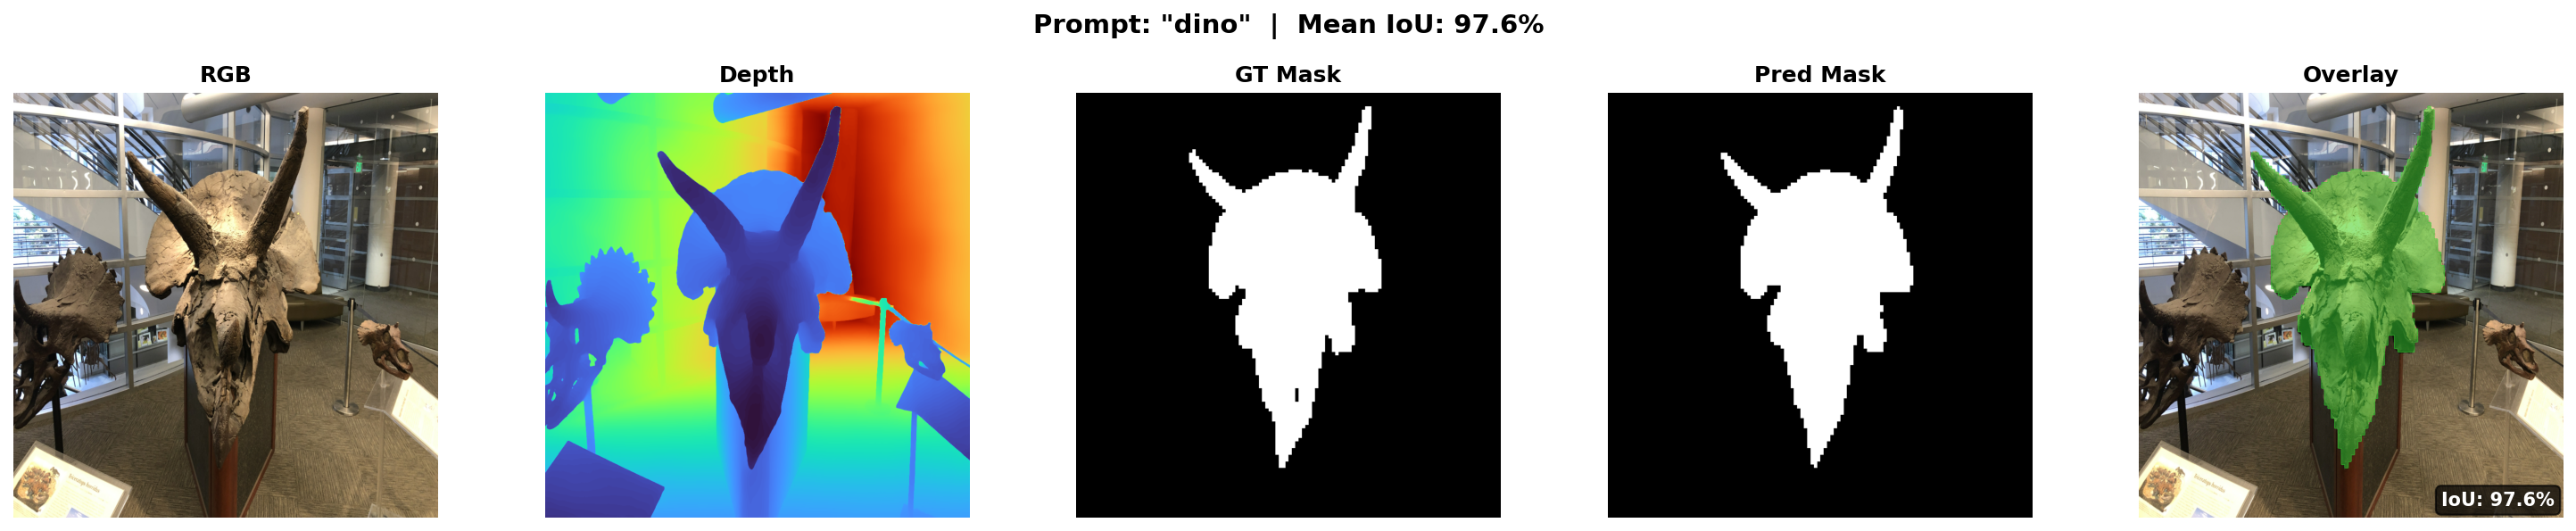
\includegraphics[width=\linewidth]{figures/nvos2.png}\\[2mm]
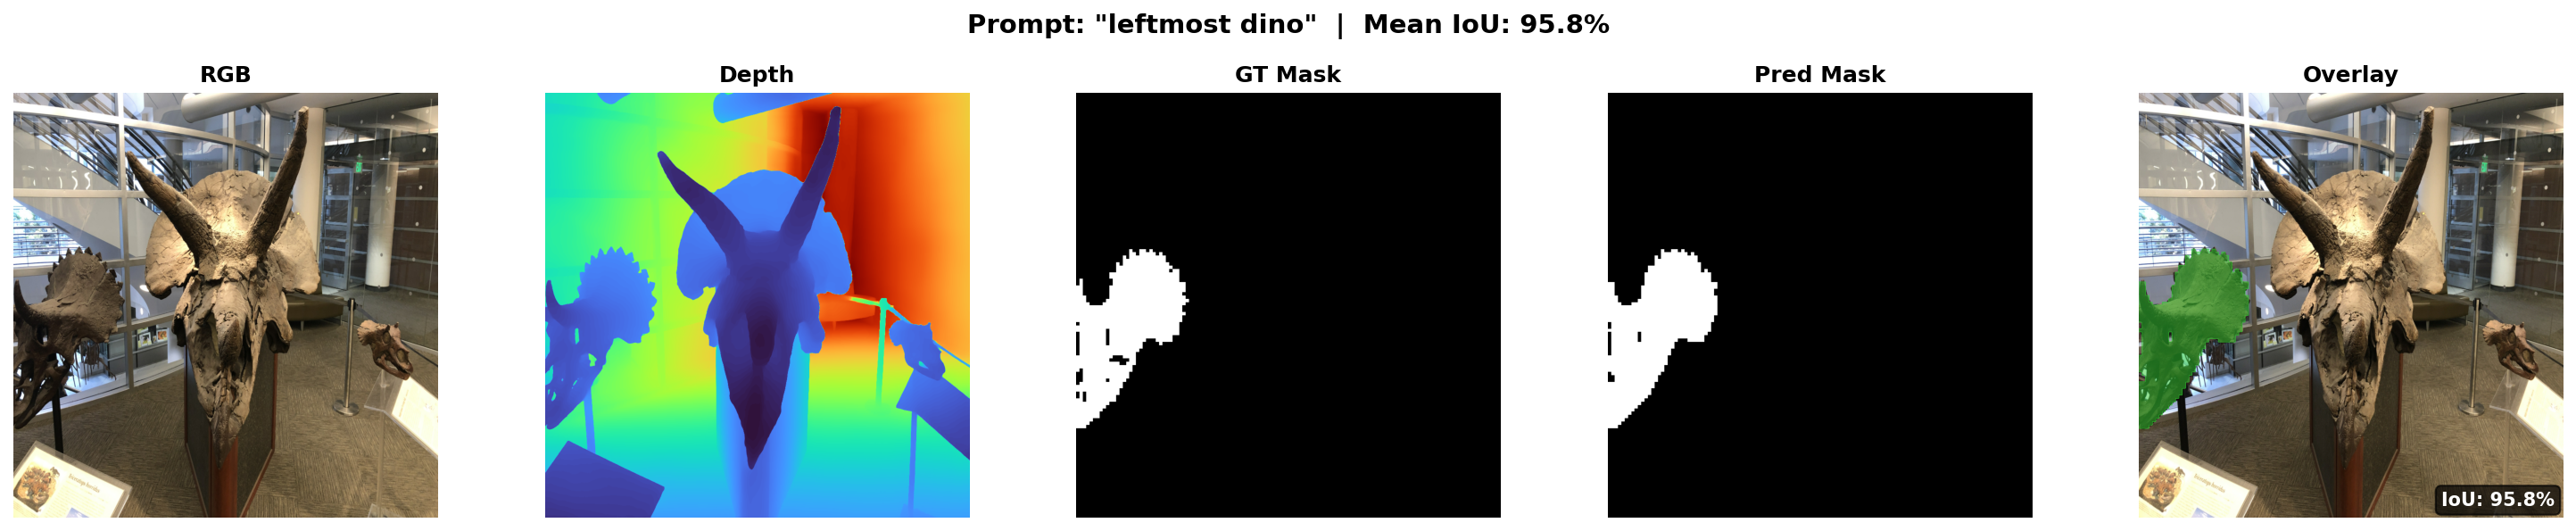
\includegraphics[width=\linewidth]{figures/nvos1.png}
\caption{Spatial disambiguation on the NVOS T-Rex scene. \textbf{Top:} The query ``dino'' (97.6\% IoU) segments the dominant triceratops skull in the scene. \textbf{Bottom:} The query ``leftmost dino'' (95.8\% IoU) leverages spatial reasoning to disambiguate between the two skulls, correctly selecting only the left specimen. The depth map (second column) provides the geometric context that enables this: TrianguLang computes 3D centroids for each candidate mask and selects the one satisfying the spatial constraint ($\arg\min_i x_i$ for ``leftmost''), resolving ambiguity that would be impossible with object names alone.}
\label{fig:nvos_trex}
\end{figure}

\begin{figure}[h]
\centering
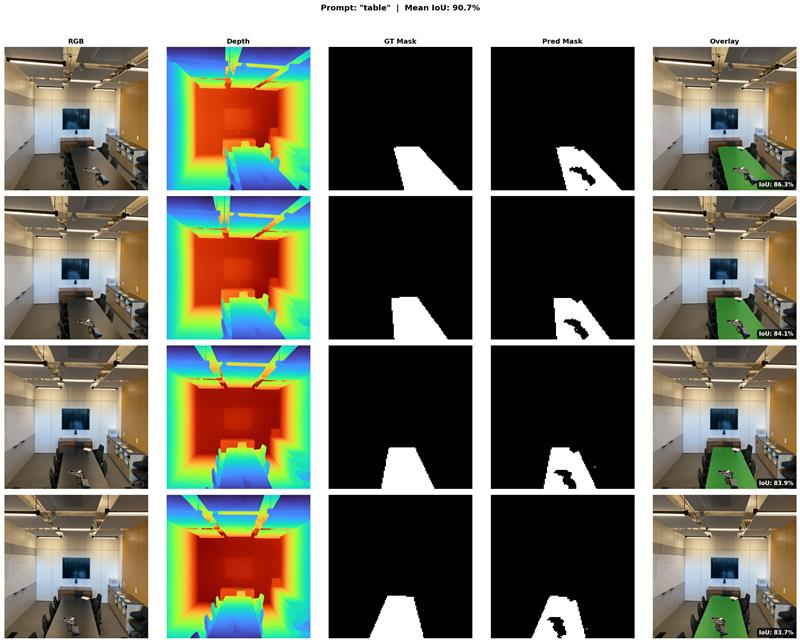
\includegraphics[width=0.9\linewidth]{figures/grid_spinnerf.jpg}
\caption{Segmentation results on the SPIn-NeRF room scene (90.7\% mean IoU). Each row shows a different viewpoint: RGB input, DA3 depth estimate, ground truth mask, predicted mask, and overlay. When queried for ``table,'' TrianguLang produces a clean segmentation of the table surface \emph{without} including the conference equipment (microphones) present in the ground truth annotation, demonstrating learned semantic boundaries rather than memorized annotation artifacts.}
\label{fig:spinnerf_table}
\end{figure}

Figure~\ref{fig:nvos_trex} demonstrates spatial disambiguation on the NVOS T-Rex scene. When queried with just ``dino,'' the model segments the dominant triceratops skull. However, when the query becomes ``leftmost dino,'' spatial reasoning activates: the model identifies all candidate masks for ``dino,'' computes their 3D centroids via depth unprojection, and selects the one with the minimum horizontal coordinate. This correctly isolates the left skull despite both specimens being semantically similar, an ambiguity that object names alone cannot resolve.

Figure~\ref{fig:spinnerf_table} illustrates a notable capability on the SPIn-NeRF room scene: when queried for ``table,'' TrianguLang produces a clean segmentation of the table surface \emph{without} including the conference equipment (microphones) that are present in the ground truth annotation. This demonstrates that our model learns semantic object boundaries rather than memorizing annotation artifacts.

\subsection{3D Mesh Reconstruction}

Figure~\ref{fig:tsdf_grid} shows TSDF mesh reconstructions extracted from TrianguLang's segmented depth maps. Given a text query, the model produces per-view masks and metric depth estimates that can be fused into a coherent 3D mesh via TSDF integration. These reconstructions demonstrate that TrianguLang's segmentations are geometrically consistent across views, enabling downstream 3D applications without per-scene optimization.

\begin{figure}[h]
\centering
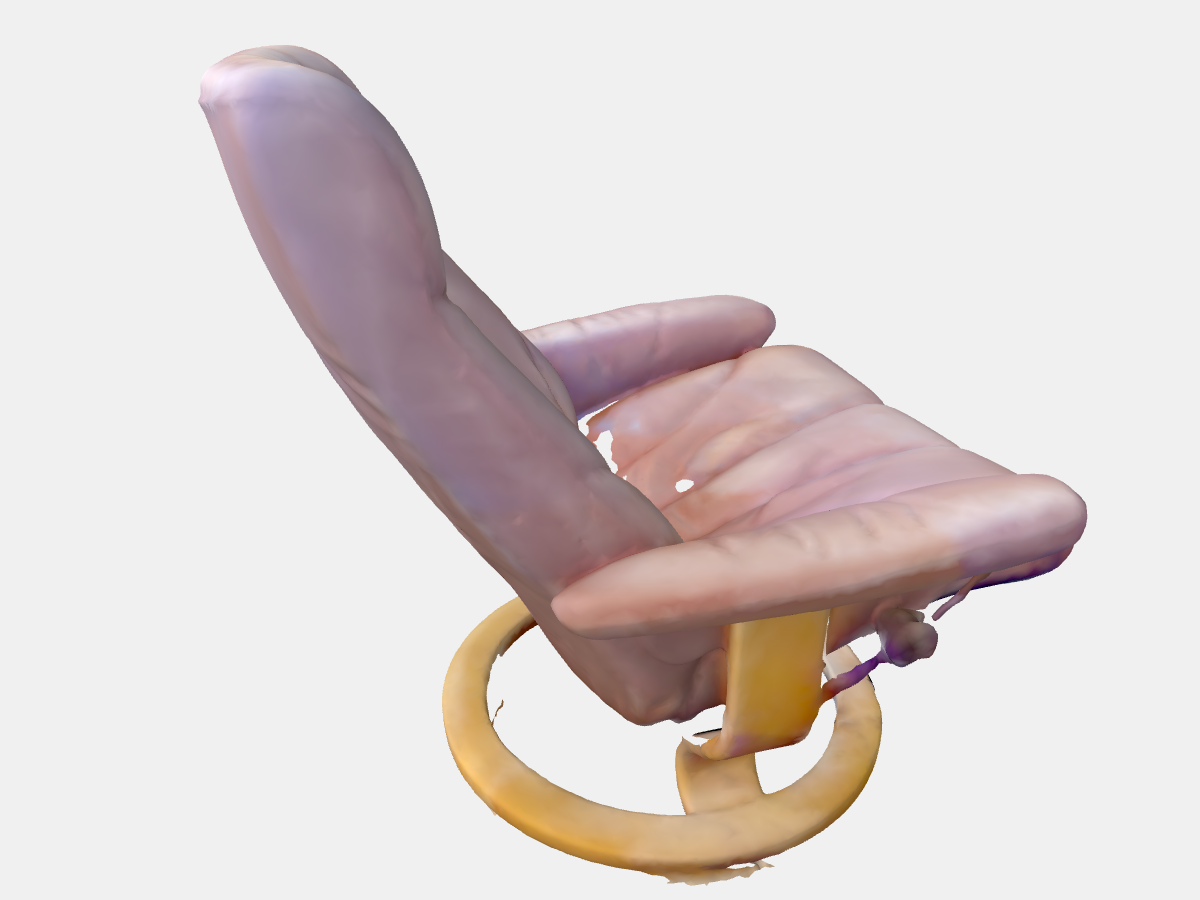
\includegraphics[width=0.32\linewidth]{figures/tsdf_sofa_chair.png}%
\hfill
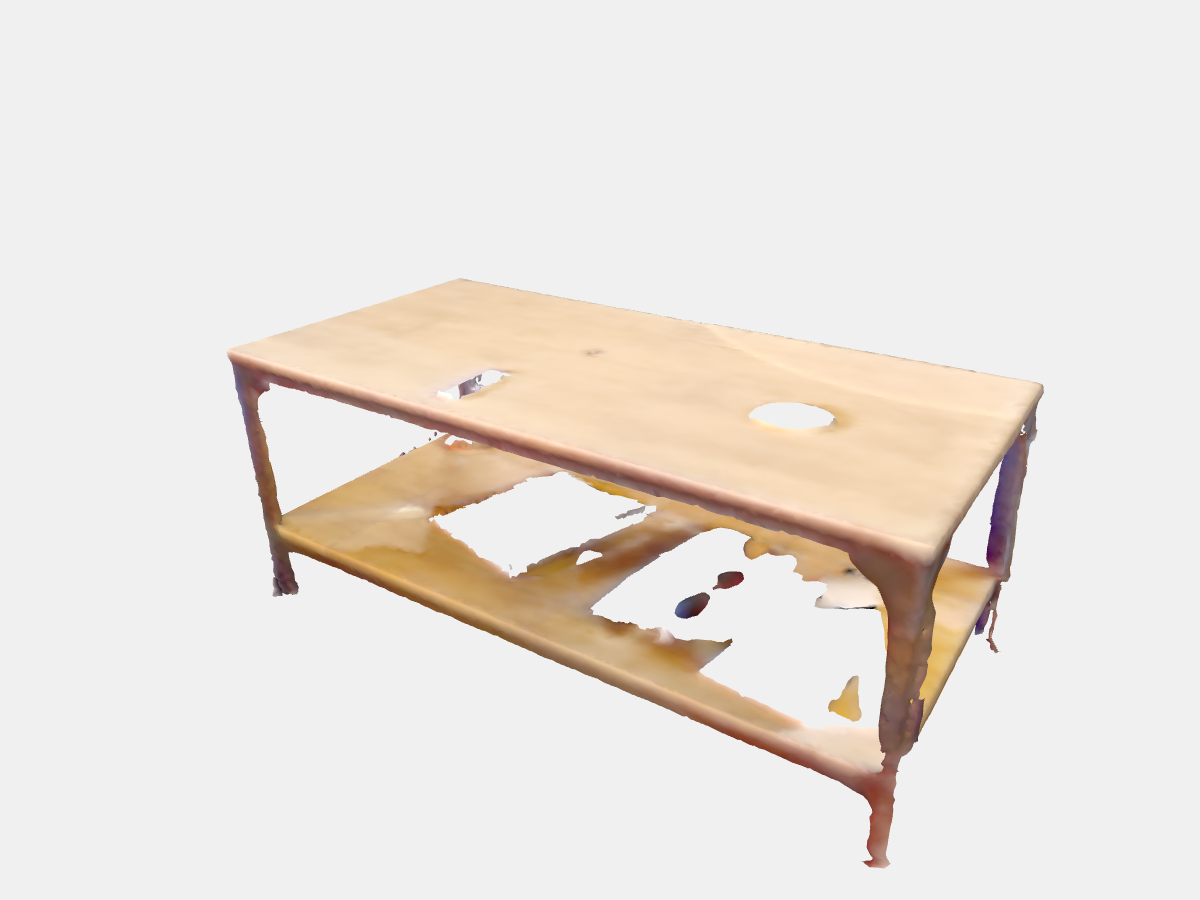
\includegraphics[width=0.32\linewidth]{figures/tsdf_coffee_table.png}%
\hfill
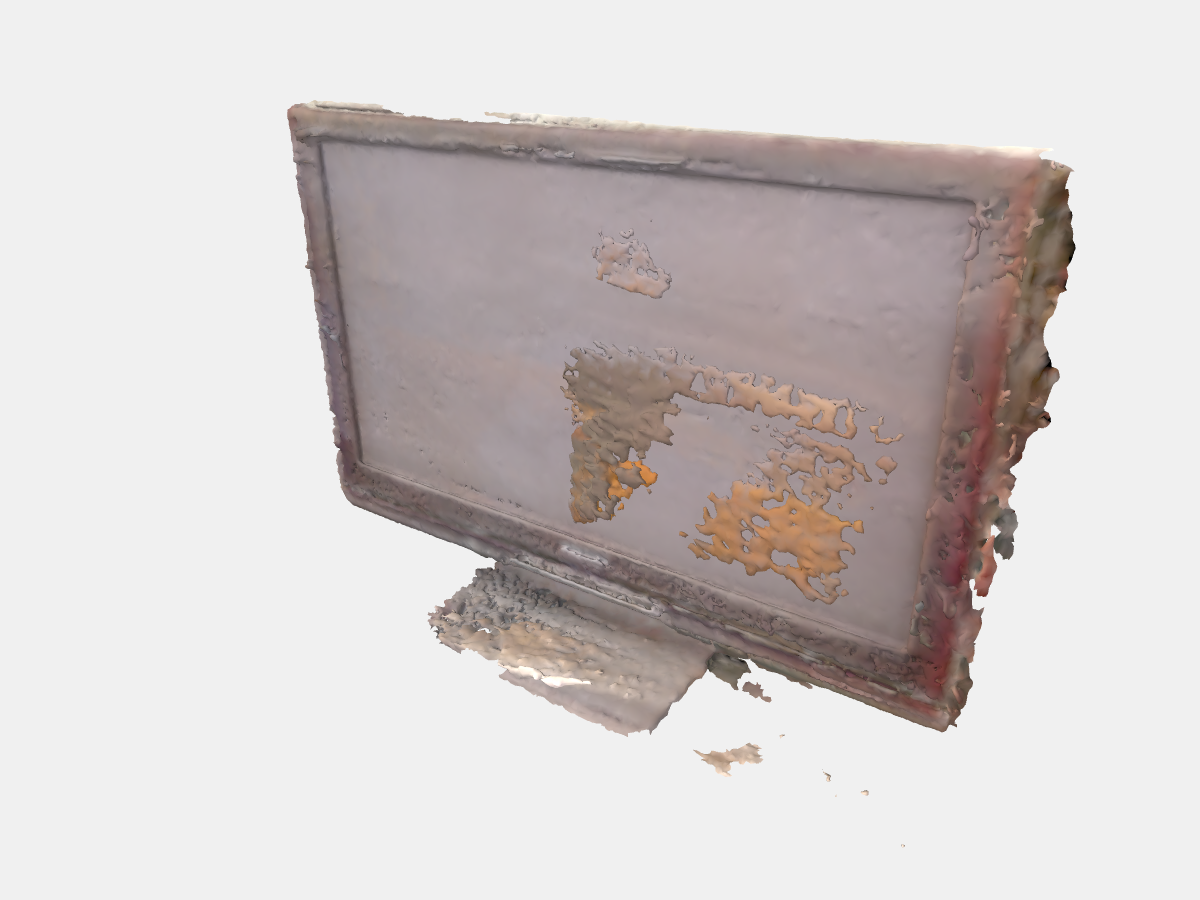
\includegraphics[width=0.32\linewidth]{figures/tsdf_tv.png}
\caption{TSDF mesh reconstructions from TrianguLang segmentations on ScanNet++ scenes. Left: ``sofa chair,'' Center: ``coffee table,'' Right: ``TV.'' Each mesh is extracted by fusing masked metric depth maps across 8 views using TSDF integration. The clean geometry demonstrates that TrianguLang produces view-consistent segmentations suitable for 3D reconstruction.}
\label{fig:tsdf_grid}
\end{figure}

